\section{Bitcoin Preliminaries}
% TODO: specific discussion of aspects of bitcoin that pertain to privacy/anonymity

In this section we introduce some common notation used in the literature involving security, privacy, and anonymity, and then present an overview of the Bitcoin system and underlying protocol for making payments (transactions). 

% \subsection{Security Definitions and Adversarial Models}

\subsection{Bitcoin Basics}

In what follows we distill a description of the Bitcoin system and underlying protocol from \cite{bitcoin}; interested readers may acquire more specific details therein if required. To begin, Bitcoin is a distributed, decentralized form of cryptocurrency. Accordingly, this enables all (digitally signed) transactions between two parties to be conducted in a peer-to-peer fashion without the inclusion of a trusted third party, such as a bank or other financial institution. This form of decentralized exchange comes at a price, however, as there must be some way to prevent users from \emph{double spending}, or using the same funds to simultaneously pay multiple parties. Bitcoin achieves this property by relying on its users to construct a history for every transaction that takes place in the system. If a majority of the users accept the validity of a particular transaction, or a set of transactions, the global history of the system is affirmatively updated and ``confirmed'' via a cryptographic hash digest that all users agree upon. This hash digest, referred to as a hash-based proof-of-work, is what constitutes the validity of the system. By the properties of the underlying hash function, the history of the system cannot be changed without breaking the function (i.e., finding collisions) or re-doing the proof-of-work, which is computationally infeasible for small groups of nodes. Therefore, so long as a majority of the Bitcoin users are honest, the system history is deemed correct and thus all signed transactions are verified, preventing double spending by potentially malicious users participating in direct, peer-to-peer transactions. 

Unfortunately, while the above scheme is semantically correct and provides strong guarantees that all financial transactions are valid, there are inherent limitations in the amount of user privacy and anonymity that can be achieved in Bitcoin. In order to adequately define these limitations, we first describe how Bitcoin transactions are generated and how the system history is maintained. For simplicity, consider the scenario in which user $A$ wants to send $N$ BTCs (Bitcoins) to user $B$. Rather than identify users by name, Bitcoin uses \emph{addresses} that are tied to specific users to use in such transactions. Denote $\mathsf{addr}_A$ and $\mathsf{addr}_B$ as the addresses of users $A$ and user $B$ used in this transaction. It is often convenient to think of Bitcoin addresses as public keys $\mathsf{pk}_A$ and $\mathsf{sf}_B$, and as such there are corresponding private keys, which we denote as $\mathsf{sk}_A$, and $\mathsf{sk}_B$, respectively.

Structurally, a transaction $T$ is a tuple comprised of the \emph{source} transactions which supplied the funds necessary to make this transaction, denoted as $\mathsf{source}$, the (public) address of the recipient, $\mathsf{addr}_B$, the amount of BTCs to send, $N$, and a digital signature of these three properties, $\mathsf{Sign}_{\mathsf{sk_A}}({\mathsf{source}, \mathsf{pk}_B, N})$. In other words, we have 
\begin{align*}
T = (\mathsf{source}, \mathsf{pk}_B, N, \sigma), 
\end{align*}
where $\sigma = \mathsf{Sign}_{\mathsf{sk_A}}({\mathsf{source}, \mathsf{pk}_B, N})$. Note that this signature is embedded in $T$ so that any other Bitcoin user may verify the validity of the content using $\mathsf{pk}_A$. Also note that $\mathsf{source}$ need not be a single transaction; user $A$ is free to use multiple transactions in order to fund their transaction to $B$. In addition to the $N$ BTC transfer from $A$ to $B$, there is often $C$ BTC amount specified in the transaction for a particular address, where $C$ denotes the amount of change that will be given to this address as a result of the transaction. It is not required that the address to which $C$ is addressed is the same as the address of $A$, though this often happens in practice. Figure \ref{fig:transaction-io} illustrates the input and output relation of our transaction from $A$ to $B$, and Figure \ref{fig:transaction-create} illustrates the steps used in constructing this transaction. Note that, in both cases, $\mathsf{source}$ is comprised of two transactions $T_1$ and $T_2$, and the resulting transaction is denoted as $T_3$.

\begin{center}
\begin{figure}
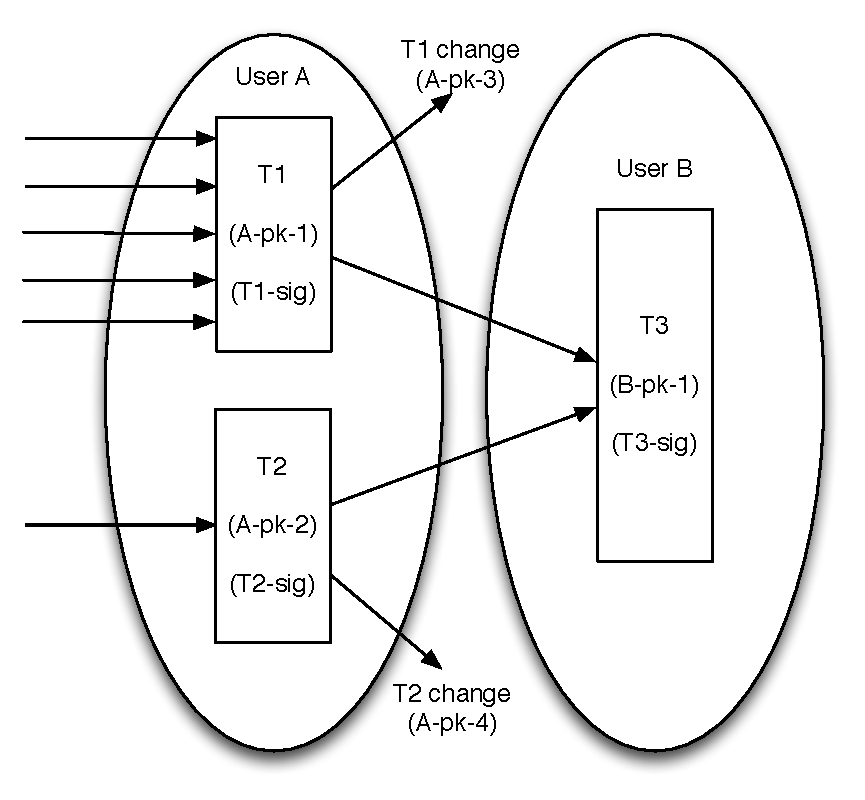
\includegraphics[scale=0.5]{./images/transaction_io.pdf}
\caption{Visual depiction of the input and output elements of a transaction from user $A$ to user $B$.}
\label{fig:transaction-io}
\end{figure}
\end{center}

\begin{center}
\begin{figure}
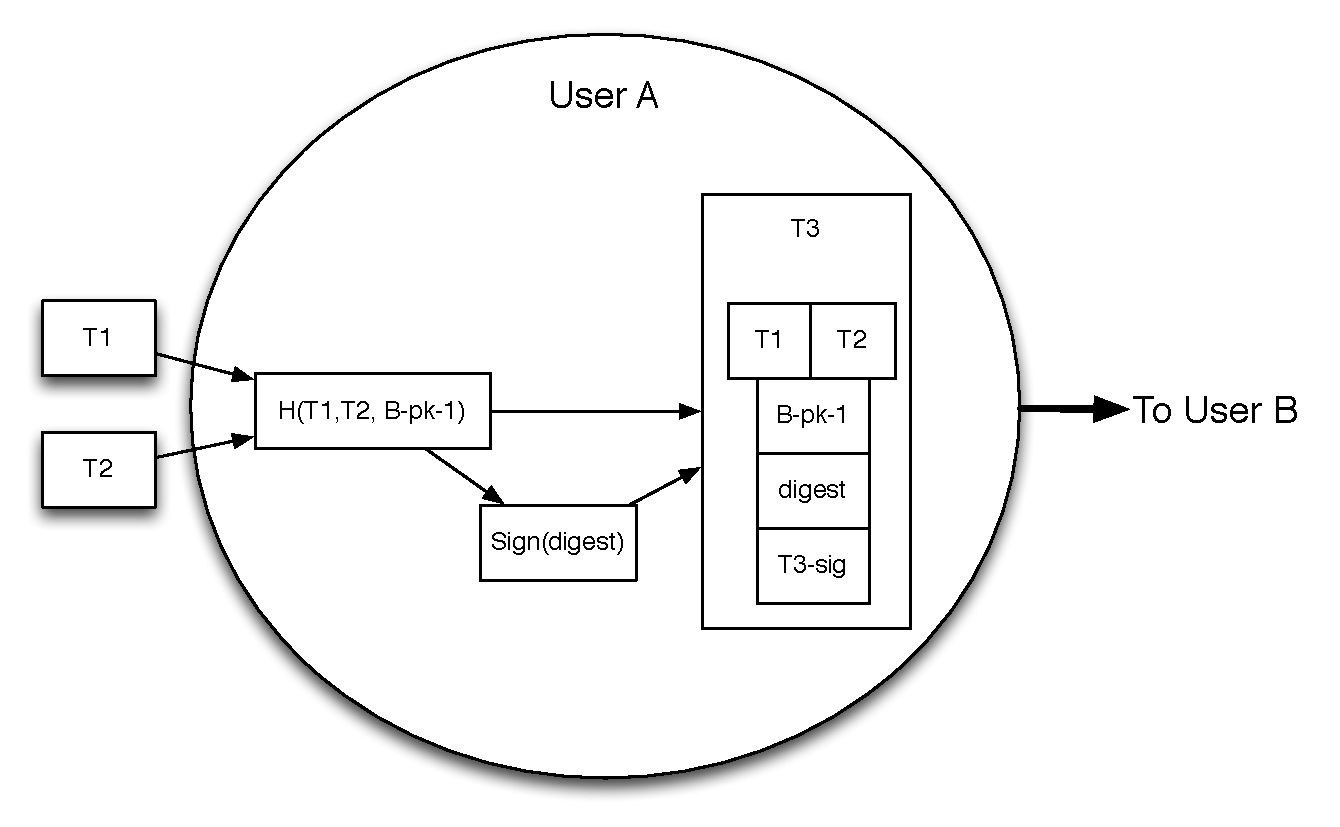
\includegraphics[scale=0.4]{./images/transaction_create.pdf}
\caption{Visual depction of the steps to create a transaction $T_3$ from user $A$ to user $B$ using two input transactions, $T_1$ and $T_2$.}
\label{fig:transaction-create}
\end{figure}
\end{center}

After a transaction has been created, it is broadcasted in the network. In order to prevent double spending, nodes must confirm this transaction and append it to the chain of accepted transactions in the system's history. This procedure is based on the aforementioned proof-of-work, which works as follows. Bitcoin miners will collect unconfirmed transactions into a buffer, along with the longest chain of system-wide accepted transactions, and compute a Merkle hash of the transactions and digest of the chain. The output digest of this Merkle hash, referred to as the challenge $c$ in the proof-of-work protocol, is then used to find the proof $p$. Together, $c$ and $p$ have the property that, when concatenated and hashed using a cryptographically strong collision-resistant hash function $H$, the leading $B$ bits of the output $x = H(c || p)$ are all $0$. That is, $x = \{0,1\}^B\{0,1\}^{256-B}$. Given the collision resistant properties of $H$, finding a valid proof $p$ for the challenge $c$ is comptuationally difficult. Figure \ref{fig:pow} illustrates the construction of $c$ and $p$ using a previously confirmed block chain $B$.

\begin{center}
\begin{figure}
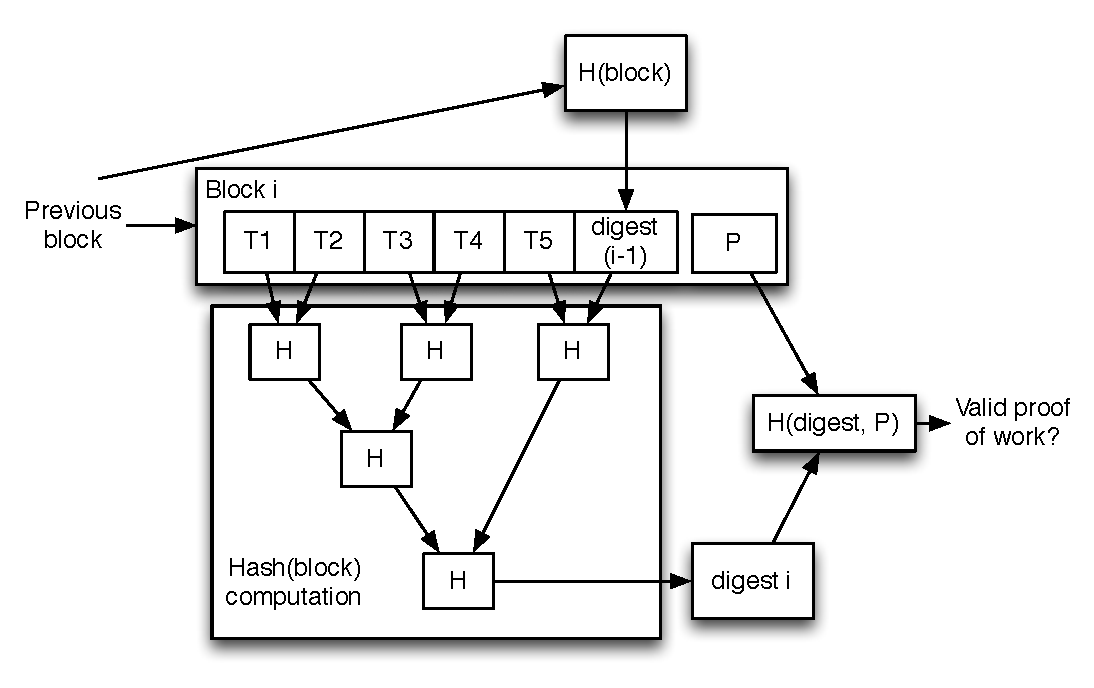
\includegraphics[scale=0.5]{./images/transaction_pow.pdf}
\caption{Proof-of-work computational procedure using the transactions of a block, the digest of the previous block, and the sampled proof $p$.}
\label{fig:pow}
\end{figure}
\end{center}

Once a miner finds a proof, it is broadcasted to the other nodes in the network along with the input transactions used by the miner, who can then easily recompute the challenge $c$ and verify the correctness of $p$. Once verified, this new transaction ``block'' is appended to the block chain which the miner used in finding the proof. Figure \ref{fig:block} illustrates a snippet of the block chain, where the challenge $c$ is the digest of the previous block and the proof $p$ are embedded in each block. Miners will continually use the longest block chain to gather and verify transaction blocks. Since there is a particular subset of BTCs in each transaction that are paid to the miner who provides the proof-of-work for a block containing that transaction, referred to as the transaction fee, miners are financially incentivized to collect more transactions into a block and continually ``mine'' for valid proofs-of-work. 

\begin{center}
\begin{figure}
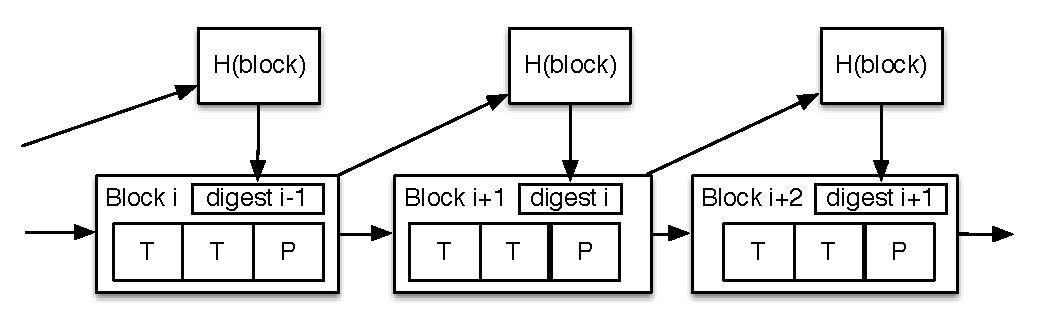
\includegraphics[scale=0.5]{./images/transaction_block_pow.pdf}
\caption{A snippet of a Bitcoin transaction block chain, illustrating the groupings of transactions into a blocks, the declaration of the proof of the work $p$, and the digest of the previous block linking the blocks together.}
\label{fig:block}
\end{figure}
\end{center}

\subsection{Bitcoin Privacy Measures}
As the topic of the survey indicates, Bitcoin has serious privacy flaws. However, there are several standard practices that Bitcoin clients and users are recommended to follow in order to improve their overall privacy and decrease the likelihood of becoming the target of privacy- or anonymity-based attacks. First, clients (and users) should specify \emph{shadow addresses} to collect change from a transaction \cite{bitcoin-shadow-addresses}. Such addresses are distinct from the user's address associated used at the time of the transaction. Furthermore, since change need not always be returned to the user who provided the BTC funds, this disjoint address obfuscates the link between the address and the original user, thus helping improve overall privacy. Secondly, it is recommended that all users maintain and continually swap their addresses, and as a result, the underlying public and private key pairs, in order to deter attacks that stem from address re-use. We discuss attacks of this nature in the following sections.

